\documentclass[a4paper, 11pt]{article} % rajouter l'option [parskip] pour supprimer l'indentation et ajouter un saut de ligne à chaque début de paragraphe (halfparskip pour une demi-ligne)
\usepackage[utf8]{inputenc}
%\usepackage[latin1]{inputenc}
%\usepackage[applemac]{inputenc} % Pour avoir droit aux accents en compilant Mac Os Roman
%\usepackage{ucs}
\usepackage[english]{babel} % Pour franciser toutes les commandes automatiques (y compris les césures)
\usepackage[T1]{fontenc} % Définit les lettres accentuées comme caractères simples, et permet notamment d'éviter certains problèmes de césures 
\usepackage{lmodern} % Optimise encore l'utilisation des caractères accentués en utilisant l'encodage de police Latin Modern
\usepackage{textcomp} % Donne accès à certains symboles comme celui de l'euro par exemple
%\usepackage{amsmath} %Utile pour certaines pinailleries mathématiques. Attention à ne pas le charger si on n'en a pas besoin car il peut modifier certains environnements comme equnarray par exemple.
%\usepackage{eurosym}
\usepackage{graphics,graphicx} 	%pour inclure des graphiques
%\usepackage{subfigure}
%\usepackage{lscape}
%\usepackage{textcomp}
%\usepackage{wrapfig}		%figure dans le texte
%\usepackage{floatflt}		%figures dans le texte
%\usepackage{picins}		%figures dans le texte

\usepackage[colorlinks,bookmarks=false,linkcolor=blue,urlcolor=blue]{hyperref} %Pour les liens internet, hypertexte, email
\usepackage{geometry}		%pour les dimensions de la page
\usepackage{fancyhdr}		%entête et pied de page personnalisés, pour plus d'info voir ``entête latex'' dans favoris
\usepackage{amsmath,amssymb} %Utile pour certains symboles mathématiques
%\setlength{\parindent}{0cm} % Pour supprimer l'indentation en début de paragraphe
%\setlength{\parskip}{\baselineskip} % Pour programmer un saut de ligne avant chaque paragraphe, solution à éviter
\usepackage{lastpage}		%pour indiquer le nombre de pages
\usepackage{multirow}		%tableau sur plusieurs lignes
\usepackage{color}		
\usepackage{url}
%\usepackage{easybmat} Pour dessiner des matrices par blocs
\usepackage{subcaption}
\usepackage{pgfplots}


%Pour inclure du code C++
\usepackage{listings}
\usepackage{xcolor}
\usepackage{amssymb}
\usepackage{animate}

% Pour le pseudo-code
\usepackage{algorithm}
\usepackage[noend]{algpseudocode}



%modification de la mise en page
\geometry{a4paper,tmargin=33mm,bmargin=33mm,lmargin=28mm,rmargin=28mm}
\setlength{\parskip}{\medskipamount} 	%saut moyen entre §
\setlength{\parindent}{0pt}		%pas de retrait
%\pagestyle{headings}        		% Pour mettre des entêtes avec les titres des sections en haut de page
\pagestyle{fancy}
\lhead{ \textsc{}} \chead{} \rhead{Marine Froidevaux} \lfoot{\today}\cfoot{\thepage} \rfoot{} \renewcommand{\headrulewidth}{0.4pt} \renewcommand{\footrulewidth}{0.4pt}


%%initialisation pour le C++
%\lstset{language=C++, tabsize=2}
%\lstset{basicstyle=\small\ttfamily,
%keywordstyle=\color{blue}\bfseries,
%commentstyle=\color{red},
%stringstyle=\color{orange}
%showstringspaces=wrong}


%Initialisation for Matlab
\lstset{language=Matlab, keywords={break,case,catch,continue,else,elseif,end,for,function,
global,if,otherwise,persistent,return,switch,try,while},
basicstyle=\ttfamily,
keywordstyle=\color{blue},
commentstyle=\color{red},
stringstyle=\color{magenta},
numbers=left, numberstyle=\tiny\color{gray},
stepnumber=1,
numbersep=10pt,
backgroundcolor=\color{white},
tabsize=3,
showspaces=false,
showstringspaces=false, frame=single}



\def \be {\begin{equation*}}
\def \ee {\end{equation*}}
\def \bee {\begin{equation}}
\def \eee {\end{equation}}
\def \bm {\begin{pmatrix}}
\def \em {\end{pmatrix}}
\def \bd {\begin{displaymath} \left[ \begin{array}}
\def \ed {\end{array} \right. \end{displaymath}}
\def \ba {\begin{displaymath} \begin{array}}
\def \ea {\end{array} \end{displaymath}}
\def \bv {\begin{verbatim}}
\def \ev {\end{verbatim}}
\def \d {\partial}
\def \i {\infty}
\def \O {\mathcal{O}}
\def \X {\mathcal{X}}
\def \R {\mathbb{R}}
\def \t {\times}
\def \rank{\mbox{rank}}
\def \Y {\mathcal{Y}}
\def \C {\mathcal{C}}
\def \Mr {\mathcal{M}_{r}}
\def \E {\mathcal{E}}
\def \Xl {\mathcal{X}_{l}}
\def \bO{\bar{\Omega}}


%\renewcommand{\thesubsubsection}{ \alph{subsubsection})}
%\renewcommand{\thesubsection}{}


\newcount\dotcnt\newdimen\deltay
\def\Ddot#1#2(#3,#4,#5,#6){\deltay=#6\setbox1=\hbox to0pt{\smash{\dotcnt=1
\kern#3\loop\raise\dotcnt\deltay\hbox to0pt{\hss#2}\kern#5\ifnum\dotcnt<#1
\advance\dotcnt 1\repeat}\hss}\setbox2=\vtop{\box1}\ht2=#4\box2}

%\makeatletter
%\renewcommand\thesubsection{}
%\renewcommand\thesubsubsection{\@arabic\c@section.\@arabic\c@subsection. \alph{subsubsection})}
%\makeatother

\makeatletter
\def\BState{\State\hskip-\ALG@thistlm}
\makeatother


\newcommand{\mail}[1]{{\href{mailto:#1}{#1}}}
\newcommand{\ftplink}[1]{{\href{ftp://#1}{#1}}}

\begin{document}
\title{Error Concealment using 3D Low-Rank Tensor Completion}%\\ \textsc{}}
%\author{Lukas König et Marine Froidevaux\\ \mail{lukasgeorg.koenig@epfl.ch} \\ \mail{marine.froidevaux@epfl.ch}}
\author{Marine Froidevaux \\ \mail{marine.froidevaux@epfl.ch} \\ \\Supervisors: Dr. Jonas Ballani and Prof. Daniel Kressner 
 }% \\ \mail{marine.froidevaux@epfl.ch}}
%\date{2011} % Si on ne met pas du tout la commande "date" le maketitle ajoute automatiquement la date du jour à la page de titre. Pour ne pas voir apparaître la date il faut écrire la commande vide \date{}.



\maketitle
%\begin{figure}[h!]
%\centering
%\includegraphics[scale=0.5]{electrode}
%\end{figure}
%
%\newpage
\thispagestyle{empty}
\pagenumbering{roman}
\setcounter{tocdepth}{2} % Pour afficher les paragraphes (profondeur 4) dans la table des matières
\tableofcontents
\newpage
\pagenumbering{arabic}



\section{Introduction}
Error concealment is a domain of image processing which deals with

Error typically in form of patches 

This report presents an error concealment algorithm, called Alternating Least Square, that reconstructs the corrupted patches by exploiting the low-rank property of a stack of similar patches. Results of the application of this algorithm to movie reconstruction and inpainting are presented here as well. 

Moreover, for comparison purpose, the same movies and images were reconstructed using the algorithm GeomCG for low-rank approximation.

\section{Basics of tensor algebra}
Before looking at the error concealment algorithm in details, a few basic tools of tensor algebra need to be defined.
This section is based on the paper by Kolda and Bader \cite{Kolda-Bader}, which should be referred back to for further details.

It is sufficient for our purpose to consider three-dimensional tensors only, but all algebraic concepts presented in this section can be generalised to higher dimensions.

Let $\X \in \R^{I_1\t I_2 \t I_3}$.
The \underline{i$^{th}$ matricisation} of $\X$ is a reordering of its entries into a matrix $X_{(i)} \in \R^{ I_i\t \prod_{j\neq i}I_j}$ such that the indices of $\X$ in the i$^{th}$ dimension become the row indices of $X_{(i)}$ and the indices of $\X$ in the other dimensions are rearranged in lexicographical order to become column indices of $X_{i}$. 

The $i-$rank of $\X$ is defined as the rank of its i$^{th}$ matricisation. The \underline{multilinear rank} of $\X$ is a 3-tuple grouping the $i$-rank of $\X$ in each of the three dimensions:
\be
\rank(\X):=\left[\rank(X_{(1)}),  \rank(X_{(2)}), \rank(X_{(3)})\right]
\ee

The \underline{i$^{th}$-mode produc}t of $\X$ with a matrix $M \in \R^{m\t I_i}$ is a tensor $\mathcal{Y} \in \R^{J_1\t J_2\t J_3}$, with $J_j=I_j$ for $j\neq i$, and $J_i=m$. $\mathcal{Y}$ is defined by means of the matricisation as follows:
\be
\mathcal{Y}=\X \t_{i} M \iff Y_{(i)}=MX_{(i)}
\ee
Note that the matricisation operation is a bijection from $ \R^{I_1\t I_2 \t I_3}$ into $\R^{ I_i\t \prod_{j\neq i}I_j}$. The product $\mathcal{Y}$ is thus uniquely determined by any of its matricisation.

The \underline{inner product} of two tensors $\X, \Y in \R^{I_1\t I_2 \t I_3}$ is the sum of the product of their entries, that is to say:
\bee
<\X,\Y>:=\sqrt{\sum\limits_{i_1=1}^{I_1}\sum\limits_{i_2=1}^{I_2}\sum\limits_{i_3=1}^{I_3} x_{i_1,i_2,i_3}y_{i_1,i_2,i_3}}
\label{innerProd}
\eee
The induced \underline{norm} $\|\X\|:=\sqrt{<\X, \X>}$ is thus a generalisation of the matrix Frobenius norm to 3 dimensions.

Any tensor $\X$ of multilinear rank $\rank(\X)=[r_1, r_2, r_3]$ can be decomposed into a core tensor $\C \in \R^{r_1\t r_2 \t r_3}$ and three orthogonal basis matrices $A_i \in \R^{I_i\t r_i}$, such that
\bee
\X=\C \t_1 A_1 \t_2 A_2 \t_3 A_3 
\label{Tucker}
\eee
This is called the \underline{Tucker Decomposition} and is the basis of the {High-Order Singular Value Decomposition} (HOSVD) algorithm. 

Note that a Tucker decomposition is not unique. Indeed, if $\X$ can be decomposed as in \autoref{Tucker} then for any $V_1\in \R^{r_1\times r_1}, V_2\in \R^{r_2\times r_2}, V_3\in \R^{r_3\times r_3}$ invertible, tho following decomposition holds as well:

\be
\X=\tilde{\C} \t_1 \tilde{A}_1 \t_2 \tilde{A}_2 \t_3 \tilde{A}_3 
\ee
where $\tilde{\C}=\C\t_1V_1 \t_2 V_2 \t_3 V_3$ and $\tilde{A}_i=A_iV_i^{-1}$.

HOSVD aims at computing a rank-$\left[R_1,R_2, R_3\right]$ approximation of a tensor $\X$ of higher rank in the Tucker format. This is done by matricising $\X$ in each dimension $i=1,2,3$ and using the $R_i$ principal left singular vectors as basis $A_i$ of the Tucker decomposition. The pseudo-code for the HOSVD procedure is given in Algorithm \autoref{HOSVD}.

\begin{algorithm}
\caption{Higher-Order Singular Value Decomposition}\label{HOSVD}
\begin{algorithmic}[1]
\Procedure{HOSVD ($\X, R_1, R_2, R_3$)}{}
%\State for $ i=1,2,3$
\For {$i=1,2,3}$
\State $A_i \gets R_i$ leading left singular vectors of $X_{(i)}$ 
\EndFor
\State $\mathcal{C} \gets \X \t_1 A_1^\top \t_2 A_2^\top \t_3 A_3^\top$
\State \Return {$\mathcal{C}, A_1, A_2, A_3$}
%\BState \emph{top}:
%\If {$i > \textit{stringlen}$} \Return false
%\EndIf
%\State $j \gets \textit{patlen}$
%\BState \emph{loop}:
%\If {$\textit{string}(i) = \textit{path}(j)$}
%\State $j \gets j-1$.
%\State $i \gets i-1$.
%\State \textbf{goto} \emph{loop}.
%\State \textbf{close};
%\EndIf
%\State $i \gets i+\max(\textit{delta}_1(\textit{string}(i)),\textit{delta}_2(j))$.
%\State \textbf{goto} \emph{top}.
\EndProcedure
\end{algorithmic}
\end{algorithm}


This procedure can be viewed as a generalisation of the matrix Singular Value Decomposition (SVD) as a truncated SVD is performed on each matricisation of $\X$ to obtain a lower rank approximation. However, in contrast to the 2-dimensional case, the HOSVD does not lead to the best rank-$\left[R_1,R_2, R_3\right]$ approximation of $\X$. Let us denote the subspace of  all 3-dimensional tensors of rank $r=\left[R_1, R_2, R_3\right]$  by  $\Mr:=\{ \mathcal{T} \in \R^{I_1\t I_2 \t I_3} | \rank(\mathcal{T})=\left[R_1,R_2, R_3\right] \}$ and let $P_{\Mr}\X$ be a best approximation of $\X$ in the subspace $\Mr$ relatively to the norm defined above. If $P_{HO}\X$ represents the result of the HOSVD procedure applied to $\X$ then the following results holds \cite{GeomCG}:
\be
\|\X-P_{HO}\X \|\leqslant \sqrt{3} \| \X-P_{\Mr}\X \|
\ee

This means that a best low-rank approximation of $\X$  is only better by a factor $\frac{1}{\sqrt{3}}$ than what is computed by means of the HOSVD procedure.

\section{Statement of the problem}
The description is made here for the case of movie reconstruction. Image inpainting can be viewed as a particular case of movie reconstruction where the number of frames is equal to 1.

Firstly, a Macro-Block (MB) grid is defined for each frame. The size of a MB, denoted by $N$, is typically  $8\t 8$ or $16\t 16$ pixels and the MB grid is shifted by half a block size in the vertical and horizontal direction of the frame. A given MB therefore typically overlaps with 8 other MBs from the same frame (see \autoref{MBs}) and a natural division of each MB into 4 sub-blocks arises. 

\begin{figure}[h!]
\centering
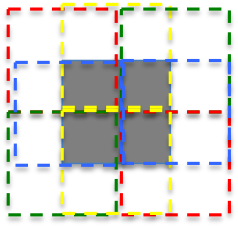
\includegraphics[scale=0.6]{MBs}
\caption{A given MB (grey) typically overlaps with 8 other MBs (red, yellow, blue and green contour) from the same frame.  \label{MBs}}
\end{figure}
%Different MBs from the same frame can therefore overlap on half of their pixels. 
\subsection{Tensor construction via selection of similar patches}

In each frame of the movie separately, all MBs containing corrupted entries are put in a list and sorted relatively to the number of clean (i.e. non-corrupted) pixels they contain.
We call $P^0$ a corrupted MB and $\Omega$ the set of its clean and concealed pixels.
$P^0$s with a larger set $\Omega$ will be reconstructed first.

Once a $P^0$ is chosen for reconstruction of its missing entries, similar MBs that are fully clean will be looked for in a some defined reference frames. We call these similar MBs $P^i$ and seek to select the $K$  $P^i$s which best match $P^0$. The best matching $P^i$ is defined as the one which minimises the error
\bee
\| P_{\Omega}^0-P_{\Omega}^i\|_1=\sum \limits_{j} |P^0_j-P^i_j|
\label{ErrorMatching}
\eee
where $j$ is an index that loops over all pixels of $\Omega$. All MBs are rescaled to have the same $L_2-norm$ as $P^0$ (on the set $\Omega$ only) before the matching error is computed. 

Note that $K$ needs to be defined as a user input, but in case less than $K$ "good matching" MBs are actually available in the reference frames, then only $K_{eff}<K$ MBs are effectively selected, in order to avoid taking into account random MBs which would pervert the results. 
In my particular implementation, any MB with an error more then twice bigger than the best matching $P^i$ was discarded from the selection.

It is important here to realise that generally the higher the number of reference frames for the selection of $P^i$s, the better the matching with $P^0$ and thus the better the reconstruction. However, the scanning of reference frames for detection of matching MBs is a very time-consuming process. The number of reference frames should therefore be a trade-off between computation time and quality of the results. 

$P^0$ and all the $P^i$s are then gathered into a 3-dimensional tensor $\X$ of size $N\t N\t K_{eff}$, where $P^0$ is the first slice of the tensor. Later in this report, $K$ will be used in place of $K_{eff}$ for the sake of simplicity, but it should be remembered that this $K$ might be smaller than the value given as user input.

\subsection{Low-rank property of the tensor}
\label{subsecIdeal}

Ideally, if the objects in the movie were not moving and the camera was keeping the same view, then $\X$ would be composed of $K$ times the same patch. It could therefore be represented as a product between the 2D patch $P$ and a constant vector 1 in the $3^{rd}$ dimension. Allowing some small sparse noise $\mathcal{E}$, it would write:
\bee
\X= \Xl+\E=P\t_3 1+\E
\label{ideal}
\eee
After decomposition of $\Xl$ int the Tucker format
\be
\X_l=\C\t_1 A_1 \t_2 A_2 \t_3 A_3
\ee
and comparison with \ref{ideal} we can write
\be
P=\C \t_1 A_1\t_2 A_2 \mbox{ and } A_3=1
\ee
In practice, $\Xl$ is not composed of $K$ exactly identical patches and its rank can thus not be 1. It is however reasonable to assume that it still has a small 3-rank. In this light, two different algorithms have been used to find a good low-rank approximation of $\X$.

\section{Description of the algorithms for low-rank approximation}
\subsection{Alternating Least Squares Algorithm (ALS)}
We call now $\bar{\Omega}$ the set of missing entries in $P^0$.

The Alternating Least Square algorithm presented in the paper by Nguyen, Dao and Tran \cite{ALS} starts by filling $P^0_{\bO}$ in the first slice of $\X$ with the mean values of the $P^i$s at these locations (see Algorithm \ref{ALS algo}, line \ref{meanPi}).

\begin{algorithm}
\caption{Alternating Least Square}\label{ALS algo}
\begin{algorithmic}[1]
%\Procedure{ALS ($\X, R_1, R_2, R_3$)}{}
\State Form $\X$ from $P^0,...,K-1$ 
\State $(\X(:,:,1))_{\bO}=(\frac{1}{K-1}\sum_{i=1}^{K-1}P^i)_{\bO}$ \label{meanPi}
\State Choose mode ranks $[R_1, R_2, R_3]$ and tolerance $\sigma_{rel}, \sigma_{it}$
\State Initialise $A_1 \in \R^{N\t R_1}, A_2\in \R^{N\t R_2}, A_3\in \R^{K\t R_3}$ randomly.
\State $A^3(:,1)=[1,...,1]^{\top}/K$ \label{here}
\For {$i=1,2,3$}
\State $\Y=\X$
\For {$j\neq i$}
	\State $\Y=\Y\t_j A_j^\top$
\EndFor
\State$Y_i\gets$  unfold $\Y$ in mode $i$
\State $A_i$=first $R_i$ principal components of $Y_i$
\EndFor
\State $\C=\X\t_1 A_1^{\top}\t_2 A_2^{\top}\t_3 A_3^{\top}$
\State $\X_l=\C\t_1 A_1 \t_2 A_2 \t_3 A_3$
\State If convergence is reached, stop ; else return to Step \ref{here}
\State Recover missing area in $P^0$: $(P^0)_{\bO}=(\Xl(:,:,1))_{\bO}$
\end{algorithmic}
\end{algorithm}

While the multilinear rank $R_3$ is supposed to be small (it was set to 3 in the following examples), no assumption can be made on $R_1$ and $R_2$. These two variables are thus generally kept to their maximal possible value $N$.

The ALS procedure is a modified version of the HOSVD presented in Algorithm \autoref{HOSVD}. It is a iterative process which updates the basis matrices $A_i$ one by one, keeping the other two constant. In this way, $A_3$ can be enforced at each iteration to fulfil an additional condition.
Indeed, in the ideal case described in \autoref{subsecIdeal}, $A_3$ was a constant vector 1. Since we look for a solution which is know to be close to the ideal case, convergence can be helped by forcing the first vector of $A_3$ to be constant and normalised to 1.

The procedure is considered to have reached convergence at iteration $n$ if one of these two conditions is fulfilled:
\begin{enumerate}
\item The low-rank tensor $\Xl^{(n)}$ has become close enough to $\X$, i.e.
\be
 \epsilon_{rel}^{(n)}:=\|\Xl^{(n)}-\X \|/\| \X\|<\sigma_{rel}
\ee
\item The change made during in 1 iteration has become negligible, i.e. 
\be
|\epsilon_{rel}^{(n)}-\epsilon_{rel}^{(n-1)}|<\sigma_{it}
\ee
\end{enumerate}

\subsection{GeomCG}
The second algorithm, GeomCG, is the one presented in the paper written by Kressner, Steinlechner, Vandereycken \cite{GeomCG}. Their implementation of the algorithm is available on their website \cite{SiteANCHP} and is the one which was used here.

The aim of GeomCG is to minimise the cost function
\be
f_{\X}(\Y)=\| P_{\Omega}\Y-P_{\Omega}\X\|^2
\ee
under the constraint $\Y \in \Mr$.

The algorithm is based on the fact that $\Mr$  is a smooth subspace of $\R^{I_1\t I_2 \t I_3}$ and that, together with the inner product (\ref{innerProd}), it forms a Riemannian manifold.
An extension of the non-linear Conjugate Gradient method is used to minimise the cost function $f_{\X}(\Y_k)$. The direction of optimisation and the step size are computed by projecting the euclidian gradient of $f_{\X}(\Y_k)$ into the tangent plan of $\Mr$ at position $\X$. After each optimisation the resulting tensor is retracted back onto $\Mr$, which ensures that the low-rank condition on $\Y$ remains satisfied.
\section{Results}

\subsection{Bus Sequence}
\subsection{Inpainting}
\subsection{Effect of the corruption ratio}

\section{Conclusion}
\section{Suggestion for further research}

\begin{thebibliography}{9}
%\bibitem{Allan} 
%Allan Nielsen. 
%\textit{Solving the shallow water wave equation on HPC hardware. MATH454 Final Project}. 
%2015.

\bibitem{ALS} 
D.T. Nguyen, M.D. Dao and T.D. Tran. {The John Hopkins University}, 2011.
\textit{Error Concealment Via 3-Mode Tensor Approximation.} 18th IEEE Conference on Image Processing


\bibitem{GeomCG} 
D.Kressner, M. Steinlechner and B.Vandereycken.{ \'Ecole Polytechnique F\'ed\'erale de Lausanne}, 2013. \textit{Low-Rank Tensor Completion by Riemannian Optimization}


\bibitem{Kolda-Bader}  T.G. Kolda and B.W. Bader. {Sandia National Laboratories}, 2009.
\textit{Tensor Decomposition and Applications}. SIAM Review, Vol.51, No.3, pp. 455-500

\bibitem{SiteANCHP} \url{http://anchp.epfl.ch/geomCG}
\end{thebibliography}

%\begin{thebibliography}{99} % Beamer does not support BibTeX so references must be inserted manually as below
%\bibitem[ALS]{} D.T. Nguyen, M.D. Dao, T.D. Tran, \textit{The John Hopkins University}, 2011
%\newblock Error Concealment Via 3-Mode Tensor Approximation
%\newblock \emph{18th IEEE Conference on Image Processing}
%
%\bibitem[GeomCG]{} D.Kressner, M. Steinlechner, B.Vandereycken, \textit{\'Ecole Polytechnique F\'ed\'erale de Lausanne}, 2013
%\newblock Low-Rank Tensor Completion by Riemannian Optimization
%
%\bibitem[Kolda-Bader]{} T.G. Kolda, B.W. Bader, \textit{Sandia National Laboratories}, 2009
%\newblock Tensor Decomposition and Applications
%\newblock \emph{SIAM Review}, Vol.51, No.3, pp. 455-500
%\end{thebibliography}
%

\end{document}